\chapter{Programmable Computer Networks}\label{sec:ch-networks}\label{chap:nets}
Computer networks serve the important function of allowing any two machines to communicate with one another, typically via individual messages know as packets (i.e., a packet-switched network).
Naturally, reality is much, much more complex than this broad statement would otherwise let on; the local routing fabric in a modern network comprises specialised (though commonplace) hardware for correctly routing these packets through arbitrary topologies of links and switches at ever-increasing data rates.
This grows more complicated still when we consider the task of \emph{inter}networking between such networks, where we must route packets on higher-level logically structured addresses between different domains of control according to fairly complex policies and relationships.
At the inception of these technologies, computing scientists of the day wisely decided that the sole duty of the network itself should be the correct routing of individual packets.
Their view was that application-level logic should be executed solely at endpoint machines; their definition extended, of course, to even include desirable (and some would say indispensable) transport-level properties such as error checking and stream reliability.
This is known as the \emph{end-to-end principle}~\parencite{DBLP:journals/tocs/SaltzerRC84}.
This position arose partly due to the logical complexity of all the tasks pushed onto the network at this time, as well as the need to ensure optimal forwarding performance while microprocessors were still relatively nascent, but was instrumental in ensuring that the network itself remained \emph{extensible}.
A consistent, pared down feature set ensured while offering a good degree of freedom for the development and deployment of higher-level protocols.

Decades have passed since then, and to a large extent the zeitgeist has shifted on just how capable our networks should be---in both the research community and operators of large-scale networks.
Consider the case where an operator has a fully converged network built entirely on fixed-function hardware, but wishes to use some program to inspect the behaviour, state, and characteristics of some flow between two local machines.
The problem is that these devices offer no means of modifying or influencing routing state, being highly-optimised switching devices that understand a selection of routing algorithms built into their internal circuitry.
For the longest time, altering the network's routing behaviour in this instance---even for a single override---required not only physically altering and rewiring the network, but also would require additional hardware.\sidenote{Revisit this later... maybe a better example will come to me?}
\gls{acr:sdn} was a key development in allowing fine-grained routing over traffic at various layers in the protocol stack, allowing operators to offer per-flow or per-class routing for improved performance---\gls{acr:te}---or even application-aware load balancers at routing level.
These have been pushed even further as the runtime capabilities of supporting devices have evolved into what we might now consider truly \glsxtrfullpl{acr:pdp}.

Although our general-purpose Internet remains much the same from an endpoint perspective, specialised networks such as those in datacentres have driven innovations in \emph{in-network compute}.
In-network compute 
?? Talk about application benefits.
?? In-network compute.

Of course, over the last 
?? Levels of engineering work at many levels of abstraction which interlink, interlock, and depend on one another

What we have now are a wide variety of ways to run programs of varying levels of complexity at ?? many levels of the stack ?? to aid application and networkr performance

\gls{acr:ebpf}, \gls{acr:xdp}~\parencite{DBLP:conf/conext/Hoiland-Jorgensen18}

later netmap~\parencite{DBLP:conf/usenix/Rizzo12}

In this chapter, I'll...
\section{From Fixed-Function to Fully-Programmable}

?? What are networks?

?? Possibly discuss the internet

?? Lead in from ARPAnet et al. (2 paras). Scientific comms -> general use,

The intro of choice~\parencite{DBLP:journals/ccr/FeamsterRZ14}

?? interconnection physical and reconfig are main challenges that made SDN look attractive, reasonable?

\section{Operation and Management}

?? network-network comms? BGP

?? IGP?

?? packets routed on a per-hop basis from their perspective: may be higher level in practice (MPLS, path switching within a gateway)

?? How can we examine this? High-level (above), mid-level ()

?? Two axes: end-to-end protocol and fabric behaviour. interact in a very delicate way (i.e., host )

?? named-data networking as potential structure of the Internet?~\parencite{DBLP:journals/ccr/0001ABJcCPWZ14}
?? Can I use this to suggest/outline problems which might be solved/encountered in a future Internet?

?? Talk about \gls{acr:as} families here: \glspl{acr:isp}, hypergiants~\parencite{DBLP:conf/sigcomm/GigisCMNKDKS21}...
?? Data centres: refer to e.g. google Espresso [sigcomm 2017] as big SDN deployments

\subsection{Fixed-Function Hardware}

\subsection{Software-Defined Networking}

?? Run through the historical context. Why? What led into P4 (OpenFlow, network operating systems...)

?? \gls{acr:ovs}~\parencite{DBLP:conf/nsdi/PfaffPKJZRGWSSA15} huge here.

?? A survey to mine for stuff~\parencite{DBLP:journals/comsur/NunesMNOT14}

?? Tie into PDP here: active networking and TPP . Think about the concept of protocol boosters~\parencite{DBLP:journals/jsac/FeldmeierMSBMR98}. (NOT READ)

\section{Traffic Characteristics}

?? Can (and should probably) discuss different traffic classes here: congestion-aware, -unaware...

?? Note, explain that this is NOT just TCP vs UDP due to existence of SCTP over UDP (See: DTLS in WebRTC), QUIC over UDP, ...

?? Chain this into \glspl{acr:cca}

?? Explain why you need what.

?? Historical context for their inclusion?

?? Discussion of evolution of traffic: what's come before, what's coming next.
?? Look for older in my old notes, but recent cite here~\parencite{DBLP:conf/anrw/BauerJHBC21}.

?? Describe all my CAIDA analysis here
?? analysis of CAIDA datasets~\parencite{caida-2018-passive}
?? congestion-aware traffic makes up at least \qtyrange{73}{82}{\percent} of packets\sidenote{\url{https://github.com/FelixMcFelix/caida-stats}}
?? Also talk about QUIC's prevalence here

\subsection{Evolution}

\subsection{Emerging Protocols}

?? QUIC~\parencite{DBLP:conf/sigcomm/LangleyRWVKZYKS17}

?? QUIC carries \gls{acr:http} traffic, mostly...

\subsection{Limitations}

\section{Problems in Modern Networks}\label{sec:problems-in-modern-networks}

\subsection{Attacks on the Internet}

?? DDoS -> split by type.

?? Other attacks?

\subsection{Scaling}

\subsection{Fairness}

\section{SFC Notes}
SafeBricks~\parencite{DBLP:conf/nsdi/PoddarLPR18} extends the prior NetBricks~\parencite{DBLP:conf/osdi/PandaHJWRS16} to take advantage of TEEs.
The main framework goals above the benefits of TEEs themselves are to protect traffic from the NF (i.e., inappropriate field/packet accesses) and protect NF source code from the framework.
The execution model is a directed graph of smaller user functions including branches etc., where each NF is given access to specific packet regions by a framework (attaching a permission set to each sub-NF at build time).
This executes as a single binary in the TCB/TEE because enclave swaps in/out are particularly costly (complete cache flushes, re-encryption etc.).
DPDK daemon in userland passes packets in (i.e., Scone below)---one executing pipeline (though surely could be multiple in theory?).
NF source code (and any pre-encrypted proprietary NF source codes) are given to \emph{trusted binary} which includes all details and attested in the same manner as the compiled program.

AuditBox adds \emph{verified routing protocols} (VRPs) to this~\parencite{DBLP:conf/nsdi/LiuSKPSS21}.
This enables routing packets \emph{between enclaved NFs} (i.e., explicitly separate machines), and ensuring that the right paths are being followed, the network is not altering packets, and the network is not reordering packets (preventing MITM).
Additionally, this allows path auditing in a way which is invisible to NFs and the network (i.e., print log for like \qty{1}{\percent} of packets).
Versus prior VRPs, this enables dynamic routing between NF segments (i.e., selective filtering to a lighter or heavier function based on local state).
Note that you can do this \emph{in one box} using SafeBricks, the novelty here pertains to adaptively routing \emph{between several boxes}.
Cost? Halves goodput vs. NetBricks.

\section{Programmable Data-Planes}

\begin{figure}
	\resizebox{\linewidth}{!}{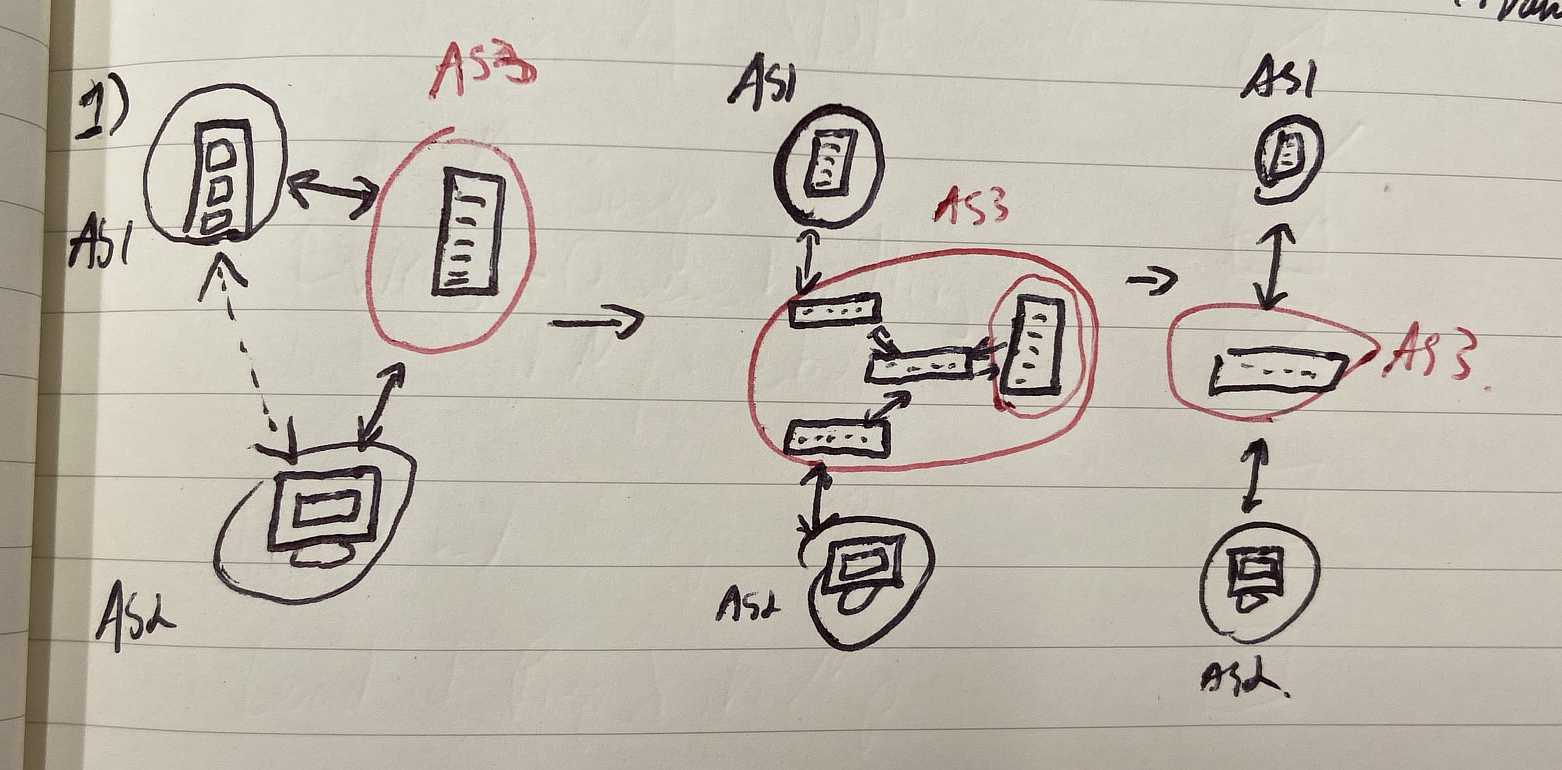
\includegraphics{diagrams/pdp-lit/steering-draft}}
	\caption{text}\label{fig:pdp-lit-steering}
\end{figure}

\begin{figure}
	\resizebox{\linewidth}{!}{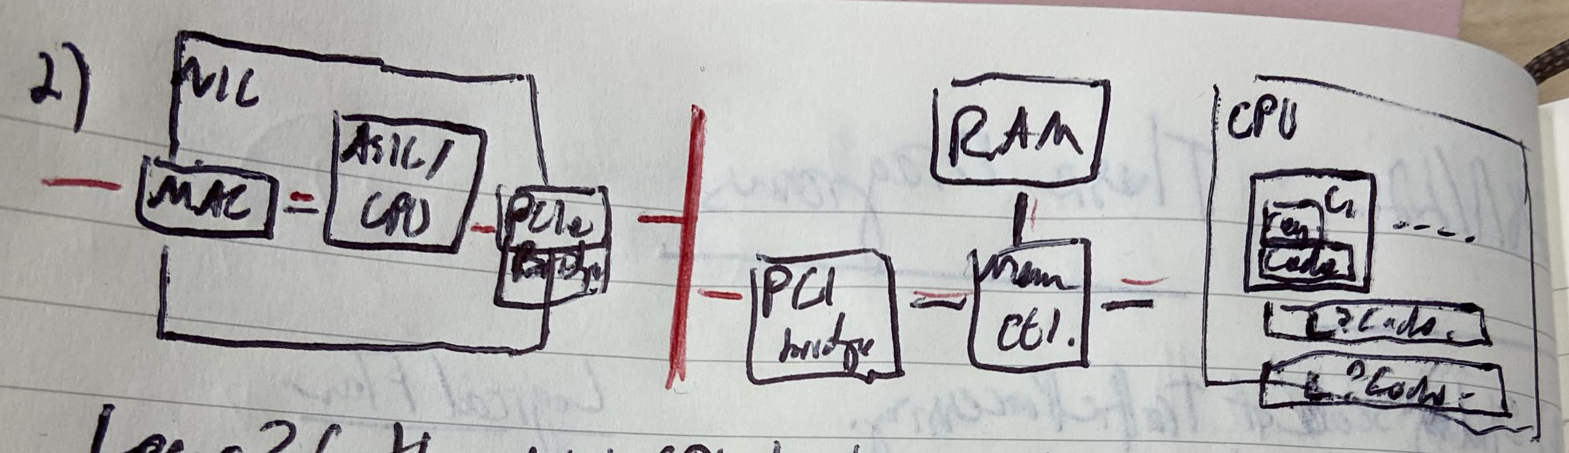
\includegraphics{diagrams/pdp-lit/pci-draft}}
	\caption{text}\label{fig:pdp-lit-pci}
\end{figure}

\begin{figure}
	\resizebox{\linewidth}{!}{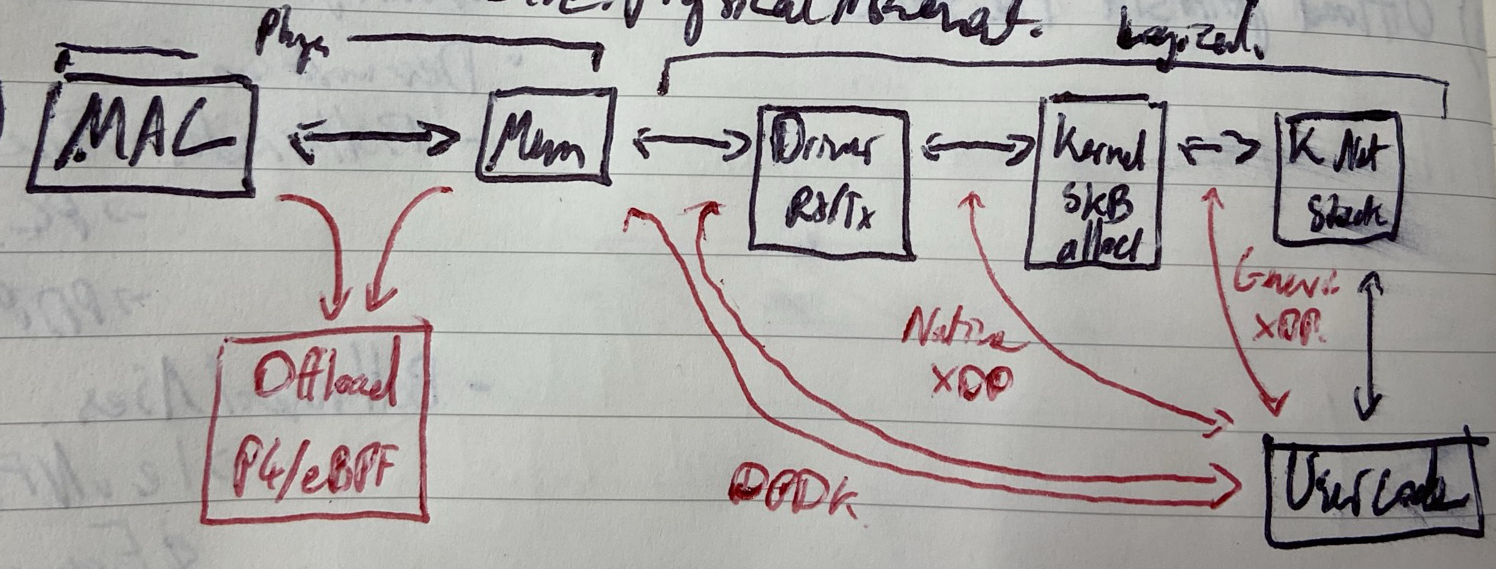
\includegraphics{diagrams/pdp-lit/offloading-draft}}
	\caption{text}\label{fig:pdp-lit-offloading}
\end{figure}

?? 2021 --- crucial to sell the why! What can be gained moving to this level, new state measures enable new applications, in-nic/switch exec reduces latencies, increases throughputs, etc...
?? Probably want a worked example showing how in-network compute helps. I.e., network graph, show processing at nodes

?? Explain \gls{acr:npu} here...

?? Understanding Host Network Stack Overheads~\parencite{DBLP:conf/sigcomm/CaiCVH021}

?? Evidence of deployment in real, huge transit networks~\sidenote{\url{https://wiki.geant.org/display/RARE/Home}, \url{https://wiki.geant.org/display/NETDEV}}

?? arbitrarily reconfigurable hardware located directly on the data path

?? OvS?~\parencite{DBLP:conf/sigcomm/TuWAP21}

?? mention how it came to this: this was an alternate solution to latency or throughput concerns which plague VNF approaches as they scale (see Metron paper for good discussion of RSS, etc., which solve these problems in their own way)

?? new ways to implement stateful + stateless packet processing.

?? History? RMT~\parencite{DBLP:conf/sigcomm/BosshartGKVMIMH13}, ClickNP, GPU offload papers. See Metron paper for cites.

?? NetFPGA~\parencite{DBLP:conf/fpga/IbanezBMZ19}

?? Getting even faster?~\parencite{nokia-fp5}

\sidenote{Test text hello.}

?? RMT was the first big innovation over OpenFlow --- read this!!

\section{Control and Management}

?? Refer back to History through OpenFlow -- what prompted the evolution?

?? Control of these devices has a lot in common with OpenFlow -- controller, except using commodity hardware to install firmwares, and so on,

\section{Software Frameworks}

\subsection{eBPF}
?? eBPF

?? BPFabric

\subsection{P4}
?? P4

?? Others who lost?

?? How do these differ? What do they share?

?? Popular frameworks now support this -- ONOS, eBPF translators, behavioural model software switch...

?? Things like Lucid built on top of P4?~\parencite{DBLP:conf/sigcomm/SonchackLRW21}

?? P4~\parencite{DBLP:journals/ccr/BosshartDGIMRSTVVW14} and \emph{programmable dataplane} (PDP) hardware~\parencite{DBLP:journals/micro/ZilbermanACM14, netronome-smartnic, xilinx-alveo, barefoot-intel}

?? Cool NIC-CPU co-design~\parencite{DBLP:conf/osdi/IbanezMAJ0KM21}

\fakepara{PDP design for asynchronous compute}
\emph{PANIC}~\parencite{DBLP:conf/hotnets/StephensAS18} places a routing fabric between distinct packet/data processing elements \emph{in a SmartNIC}.
Such designs would enable general, asynchronous, and novel compute in SmartNICs and switches, for instance offering consistent and easy to use communication between workers versus hard-coded ME relationships.
Event-driven versions of P4 have been suggested~\parencite{DBLP:conf/hotnets/IbanezABM19}.
Timer events and device state changes would empower in-network RL use-cases, signalling timesteps for RL agents or new, effective, fine-grained sources of input state.

\section{Offloading frameworks}
\emph{ClickNP}~\parencite{DBLP:conf/sigcomm/LiTLPLXXC16} targets NetFPGAs: DAG of predefined Click-like blocks, i.e. VHDL segments.
Why?
The C$\rightarrow$VHDL pipeline leads to awful code, so this achieves better FPGA usage.

\emph{Floem}~\parencite{DBLP:conf/osdi/PhothilimthanaL18} presents a DSL in python, which compiles to C for host and specific target NIC.
This does require specific dev effort per-target-NIC.

\emph{iPipe}~\parencite{DBLP:conf/sigcomm/LiuCSKPG19} runs C language programs on SmartNIC (intended) and host (emergency) according to whether traffic is at-risk of suffering from SmartNIC resource contention.
Processing is dynamically `unoffloaded' back to the host machine if SmartNIC load is too great.
This requires identical language support on both accelerator and host---which is very much not guaranteed.

\emph{hXDP}~\parencite{DBLP:conf/osdi/BrunellaBBPSBCP20} allows eBPF execution on FPGA---supports expanded eBPF ISA rather than converting program into a complete pipelined circuit (i.e., this runs as a coprocessor).
Why?
Fast redesign/reinstall time: a complete circuit bake takes ages, while JITing and compiling an eBPF program into their new ISA is pretty fast.
This includes some very cool details on around VLIW instruction-level parallelism built into their ISA and figured out during compile-time.

\emph{Gallium}~\parencite{DBLP:conf/sigcomm/ZhangZK20} converts a C++ (ClickNF program)$\rightarrow$auto-leverage PDP (P4 + C++ + P4).
Split into pre- and post-host P4 segments, with a host C++ program.
Gallium uses LLVM IR to determine read-write dependencies between variables/basic-blocks, account for PDP capabilities of packet reads (i.e., PDP can't touch packet body past $\sim$\qty{300}{\byte}), can move about \qty{100}{\byte} metadata between sites.
Identifies fast/slow paths if offloading can be elided.
Main drawback is that some annotation needed to translate Click primitives into MATs etc., otherwise the conversion to P4 means minimal additional work per target accelerator.

\emph{Flightplan}~\parencite{DBLP:conf/nsdi/SultanaSGPHSBDL21} splits P4 program into subchunks placed and routed between \{PDP, FPGA, host, server, NPU, ASIC\} for pipelining (i.e., performance) or redundancy.
Their disaggregation inserts blocks before and after splits to handle metadata (state) passing.
Their compiler breaks the programs on basic blocks with user annotations, where specific implementations manually given for some \texttt{extern}s to enable device-specific acceleration.
Data dependencies between basic blocks are extracted from the P4 IR in P4C compiler.

Preliminary work on splitting eBPF programs between an XDP part and userland part has been proposed~\parencite{DBLP:conf/conext/ShahinfarMSSBA21}.
This considers both horizontal (i.e., chunks in driver with XDP tail-calls) or vertical (user$\leftrightarrow$kernel) splits of code.
I think their XDP vs.~AF\_XDP split test confirms that the first handler in the XDP hook is basically single-threaded, which probably has some implications for our use of it as an offload.

\paragraph{Misc P4 translations.}
T4P4S~\parencite{DBLP:conf/hpsr/VorosHKLTL18} converts P4 programs into C, which are linked against a target-specific network hardware abstraction layer.
This seems to be the most effective host deployment for P4 at the moment, since it buys you DPDK-capable P4 dataplane installation compared to how terribly slow BMv2 is known to be.
Slower than native DPDK, but outpaces OvS, and allows definition of HAL binaries in SmartNIC C code as needed too.

$\mu$P4~\parencite{DBLP:conf/sigcomm/SoniR0DF20} extends P4C to decompose parser and action code into independent subprograms, to simplify porting behaviours between different switch models (V1Model, PSA, SUME, ...).

Lyra~\parencite{DBLP:conf/sigcomm/GaoZLMZTSCZY20} is a language for running Network Programming Language friendly programs (i.e., same constraints as P4 programs) across heterogeneous switch hardware, plus placement constraints.

?? P4 Verification~\parencite{DBLP:conf/sigcomm/TianGLZCZDYMTLW21}---also shows use of \gls{acr:pdp} switches in real large-scale networks (\gls{acr:isp}?)

\section{Use Cases}

?? On-switch (Tofino) DDoS detection and defence \url{https://www.usenix.org/conference/usenixsecurity21/presentation/liu-zaoxing}

\subsection{In-Network Computation}\label{sec:in-network-computation}
?? In-network computation.\sidenote{Test text hello.}

iSwitch~\cite{DBLP:conf/isca/LiLYCSH19} uses programmable switches to combine model updates between RL agents acting as part of a distributed RL training system.
Note that we discuss this in section \ref{sec:wtf}.\sidenote{Make sure that this is properly explained in the PDP seciton: source is `report-yr2.tex'.}

?? Taurus moved out of representations section~\parencite{DBLP:journals/corr/abs-2002-08987}

?? A recent line of research in the community has been to investigate \emph{Binarised/Bitwise Neural Networks} (BNNs)~\parencite{DBLP:conf/nips/HubaraCSEB16,DBLP:journals/corr/KimS16,DBLP:journals/corr/MiyashitaLM16} for line-rate packet classification.
?? \emph{BaNaNa SPLIT} shows this as an offload mechanism~\parencite{DBLP:conf/sigcomm/SanvitoSB18,DBLP:journals/corr/abs-1801-05731}; DNN inference is often carried out on the \emph{CPU} to reduce latency imposed by GPU batching and transfer, but fully-connected layers can be accelerated further by NICs.

\subsection{Network Telemetry}
?? Others (try to avoid DDN cases here).

?? The P4 ecosystem already presents novel, openly-available, fine-grained traffic measurement techniques that can be installed and controlled with ease~\parencite{DBLP:conf/sigcomm/GuptaHCFRW18,DBLP:conf/sigcomm/ChenFKRR18,DBLP:conf/sosr/GhasemiBR17}

\subsection{Transport Layer Optimisation}
?? Hi~\parencite{DBLP:conf/nsdi/ArashlooLGRWW20} Network stacks being moved into NICs to reduce latency/CPU utilisation, mainly for datacentre use-cases---otherwise, \SI{100}{\giga\bit\per\second} can't be hit. New API \emph{Tonic} for transport layer in user code (send, data management), DMA to NIC and let it handle all (de)packetisation. ``Transport logic'' goes to Tonic. Main design is datacentres, so not very high BDPs (long-fat) $\rightarrow$ \si{\kilo\byte} inflight data.

\subsection{Active Queue Management}
Turns out that you can't just write it in P4, you need to co-design for the target environment---with meaningful performance cost to boot, based on the tradeoffs you need to make~\parencite{Kunze-P4-AQM}.

\subsection{KV Stores}
NetChain~\parencite{DBLP:conf/nsdi/JinLZFLSKS18}.

\subsection{ML in PDP}
?? ML in the dataplane~\parencite{DBLP:conf/hotnets/XiongZ19,DBLP:conf/sigcomm/SanvitoSB18,DBLP:journals/corr/abs-1801-05731,DBLP:journals/corr/abs-2009-02353,langlet-ml-netronome,DBLP:journals/corr/abs-2002-08987}

\section{Hardware Designs}

?? Mention FPGA vs many-core

?? P4 etc. can actually all run on commodity hardware, which offers a third (suboptimal) hardware class.

?? Ref the paper that Haruna presented \parencite{DBLP:conf/icc/MafiolettikDMRV20}: pareto front of work-division optimality for SmartNICs (i.e., addition of high-latency cores).

?? How do these limit and influence what code can be run on different device classes? The time taken to adapt the network?

\subsection{Models of Parallelism}

\subsection{Flexibility}

\subsection{Mapping Software Frameworks}

\section{Summary}
Eh.
